\documentclass[english]{article}
\usepackage{notestemplate}
\usepackage{for}

\begin{document}

\makecover{Foundation of Operations Research}{2022/2023}

% TODO find a title for all the properties

\section{Introduction}

\subsection{Algorithm}

An algorithm for a problem is a sequence of instructions that allows to solve any of its instances.
The execution time of an algorithm depends on various factors, most notably the instance and the computer.

\bigskip
\textbf{Properties}:

\begin{itemize}
  \item An algorithm is \textbf{exact} if it provides an optimal solution for every instance.
        \begin{itemize}
          \item otherwise is \textbf{heuristic}
        \end{itemize}
  \item A \textbf{greedy algorithm} constructs a feasible solution iteratively, by making at each step a \textit{locally optimal} choice, without reconsidering previous choices
        \begin{itemize}
          \item for most \textit{discrete optimization problems}, greedy type algorithms yield a feasible solution with no guarantee of optimality
        \end{itemize}
\end{itemize}

\subsection{Dynamic Programming}

Proposed by \textit{Richard Bellman} in \(1950\), \textbf{dynamic programming} \textit{(or \DP)} is a method for solving optimization problems, composed of a sequence of decisions, by solving a set of recursive equations.

\DP is applicable to any sequential decision problem, for which the optimality property is satisfied;
as such, it has a wide range of applications, including scheduling, transportation, and assignment problems.


\subsection{Complexity of algorithms}

In order analyze an algorithm, it's necessary to consider its complexity as a function of the size of the instance \textit{(the size of the input)}, independently of the computer;
the complexity is defined as the number of elementary operations by assuming that each elementary operation takes a constant time.

Since it's hard to determine the exact number of elementary operations, an additional assumption is made: only the asymptotic number of elementary operations in the worst case (for the worst instances) is considered.
The complexity evaluation is then performed by looking for the function \(f(n)\) that best approximates the upper bound on the number of elementary operations \(n\) for the worst instances.

\subsubsection{Big-O notation}

A function \(f\) if order of \(g\), written \(f(n) = \bigO{g(n)}\) if exists a constant \(c > 0\) and a constant \(n_0 > 0\) such that \(f(n) \leq c \cdot g(n)\) for all \(n \geq n_0\).

An illustration of the big-O notation is shown in Figure~\ref{fig:big-o-notation}.

\begin{figure}[htbp]
  \bigskip
  \centering
  \tikzfig{figure-1.tikz}
  \caption{Big-O notation}
  \label{fig:big-o-notation}
  \bigskip
\end{figure}

\subsection{Complexity classes}

Two classes of algorithms are considered, according to their worst case order of complexity:

\begin{itemize}
  \item \textbf{Polynomial}: \(\bigO{n^d}\) for a constant \(d > 0, d \in \mathbb{R}\)
  \item \textbf{Exponential}: \(\bigO{d^n}\) for a constant \(d > 0, d \in \mathbb{R}\)
\end{itemize}

Algorithms with a hight order Polynomial complexity are not considered efficient.

A comparison of the two classes, assuming that \(1 \, \mu s\) is needed for each elementary operation, is shown in Table~\ref{tab:complexity-classes}.

\begin{table}
  \centering
  \bigskip
  \begin{tabular}{c|c|c}
    \(n\)  & \(n^2\)          & \(2^n\)                \\
    \hline
    \(1\)  & \(1 \, \mu s\)   & \(1 \, \mu s\)         \\
    \(10\) & \(100 \, \mu s\) & \(1.024 \, ms\)        \\
    \(20\) & \(400 \, \mu s\) & \(\approx 1.04\, s\)   \\
    \(30\) & \(900 \, \mu s\) & \(\approx 18 \, m\)    \\
    \(40\) & \(1.6 \, ms\)    & \(\approx 13 \, d\)    \\
    \(50\) & \(2.5 \, ms\)    & \(\approx 36 \, y\)    \\
    \(60\) & \(3.6 \, ms\)    & \(\approx 36535 \, y\) \\
  \end{tabular}
  \caption{Complexity classes}
  \label{tab:complexity-classes}
  \bigskip
\end{table}

\clearpage

\section{Graph and Network Optimization}

Many \textbf{decision making problems} can be formulated in terms of graphs and networks, such as:

\begin{itemize}
  \item \textbf{transportation} and \textbf{distribution} problems
  \item \textbf{network design} problems
  \item \textbf{location} problem
  \item timetable \textbf{scheduling}
  \item \ldots
\end{itemize}

\subsection{Graphs}

A \textbf{graph} is a pair \(G = (N, E)\) with:

\begin{itemize}
  \item \(N\) a set of \textbf{nodes} or \textbf{vertices}
  \item \(E \subseteq N \times N\) a set of \textbf{edges} or arcs connecting them pairwise
        \begin{itemize}
          \item an edge connecting nodes \(i\) and \(j\) is represented by \(\{i, j\}\) if the graph is \textbf{undirected}
          \item an edge connecting nodes \(i\) and \(j\) is represented by \((i, j)\) if the graph is \textbf{directed}
        \end{itemize}
\end{itemize}

\bigskip
\textbf{Properties}:

\begin{itemize}
  \item Two \textbf{nodes} are \textbf{adjacent} if they are connected by an edge
  \item An \textbf{edge} \(e\) is \textbf{incident} in a node \(v\) if \(v\) is an \textbf{endpoint} of \(e\)
        \begin{itemize}
          \item \textbf{undirected} graphs: the degree of a node is the number of incident edges
          \item \textbf{directed} graphs: the in-degree \textit{(out-degree)} of a node is the number of arcs that have it as successor \textit{(predecessor)}
        \end{itemize}
  \item A \textbf{path} from \(i \in N \text{ to } j \in N\) is a sequence of edges
        \[ p = \left\langle \{v_1, v_2\}, \{v_2, v_3\}, \ldots, \{v_{k-1}, v_k\}\right\rangle \]
        connecting nodes \(v_1, \ldots, v_k\), with \(\{v_i, v_{i+1} \in E\}\) for \(i = 1, \ldots, k-1\)
  \item A \textbf{directed path} \(i \in N \text{ to } j \in N\) is a sequence of arcs
        \[ p = \left\langle (v_1, v_2), (v_2, v_3), \ldots, (v_{k-1}, v_k)\right\rangle \]
        connecting nodes, with  \((v_i, v_{i+1} \in E)\)  for \(i = 1, \ldots, k-1\)
  \item Nodes \(u\) and \(v\) are \textbf{connected} if exists a path connecting them
  \item A graph \((N, E)\) is \textbf{connecting} if \(u, v\) are connecting \(\forall \, u, v \in N\)
  \item A graph \((N, E)\) is \textbf{strongly connected} if \(u, v\) are connected by a directed path \(\forall \, u, v \in N\)
  \item A graph is \textbf{bipartite} if there is a partition \(N = N_1 \cup N_2, \, N_1 \cap N_2 = \emptyset\) such that \(\forall \, (u, v) \in E, u \in N_1 \text{ and } v \in N_2\)
  \item A graph is \textbf{complete} if \(E = \left\{\{v_i, v_j\} \,|\, v_i, v_j \in N \land i \leq j \right\}\)
  \item Given a directed graph \(G = (N, A)\) and \(S \subseteq N\), the \textbf{outgoing cut} induced by \(S\) is the set of arcs:
        \[\delta^+(S) = \left\{ (u, v) \in A \,|\, u \in S \land v \in N \setminus S \right\}\]
        the \textbf{incoming cut} induced by \(S\) is the set of arcs:
        \[\delta^-(S) = \left\{ (u, v) \in A \,|\, v \in S \land u \in N \setminus S \right\}\]
\end{itemize}

\bigskip
Some examples are shown in Figure \ref{fig:examples-of-graphs}.

\bigskip
\textbf{Properties of graphs}:
\begin{itemize}
  \item A graph with \(n\) \textbf{nodes} has at most \(m = \dfrac{n(n-1)}{2}\) \textbf{edges}
  \item A \textbf{directed} graph with \(n\) \textbf{nodes} has at most \(m = n(n-1)\) \textbf{arcs}
        \begin{itemize}
          \item a graph is \textbf{dense} if \(m \approx n^2\)
          \item a graph is \textbf{sparse} if \(m \ll n\)
        \end{itemize}
\end{itemize}

\begin{figure}
  \centering
  \begin{subfigure}[t]{0.495\textwidth}
    \centering
    \begin{tikzpicture}[circle, node distance = 2cm, minimum size = 0.75cm]
      \samplegraph
      \sampleedges
    \end{tikzpicture}
    \caption{Undirected graph}
    \label{fig:undirected-graph}
  \end{subfigure}
  \begin{subfigure}[t]{0.495\textwidth}
    \centering
    \begin{tikzpicture}[circle, node distance = 2cm, minimum size = 0.75cm]
      \samplegraph
      \samplearcs
    \end{tikzpicture}
    \caption{Directed graph}
    \label{subfig:directed-graph}
  \end{subfigure}
  \bigskip
  \begin{subfigure}[t]{0.495\textwidth}
    \centering
    \begin{tikzpicture}[circle, node distance = 2cm, minimum size = 0.75cm]
      \samplegraph

      \path[-] (1) edge (2);
      \path[-] (1) edge (4);
      \path[-][color=red] (2) edge (3);
      \path[-] (2) edge (4);
      \path[-][color=red] (3) edge (4);
      \path[-] (3) edge (5);
      \path[-][color=red] (4) edge (5);
    \end{tikzpicture}
    \caption{\shortstack{Connected graph, nodes \(2\) and \(5\) are connected \\ \(\langle \{2, 3\}, \{3, 4\}, \{4, 5\} \rangle\) is a path}}
    \label{subfig:connected-graph}
  \end{subfigure}
  \begin{subfigure}[t]{0.495\textwidth}
    \centering
    \begin{tikzpicture}[circle, node distance = 2cm, minimum size = 0.75cm]
      \samplegraph

      \path[->] (1) edge (2);
      \path[->] (1) edge (4);
      \path[->, color=red] (2) edge (3);
      \path[->, color=red] (3) edge (4);
      \path[->, color=red] (3) edge (5);
      \path[->, color=red] (4) edge (2);
      \path[->] (4) edge[bend left=15] (5);
      \path[->, color=red] (5) edge[bend left=15] (4);
    \end{tikzpicture}
    \caption{\shortstack{Not strongly connected graph \\ \(\langle \{3, 5\}, \{5, 4\}, \{4, 2\}, \{2, 3\}, \{3, 4\} \rangle\) is a directed path}}
    \label{subfig:not-strongly-connected-graph}
  \end{subfigure}
  \bigskip
  \begin{subfigure}[t]{0.495\textwidth}
    \centering
    \begin{tikzpicture}[circle, node distance = 2cm, minimum size = 0.75cm]
      \samplegraph

      \path[-] (1) edge (2);
      \path[-] (1) edge (4);
      \path[-, color=red] (2) edge (3);
      \path[-, color=red] (2) edge (4);
      \path[-] (3) edge (4);
      \path[-, color=red] (3) edge (5);
      \path[-, color=red] (4) edge (5);
    \end{tikzpicture}
    \caption{\shortstack{Cycle \\ \(\langle \{2, 3\}, \{3, 5\}, \{5, 4\}, \{4, 2\}\rangle\) is a cycle}}
    \label{subfig:cycle}
  \end{subfigure}
  \begin{subfigure}[t]{0.495\textwidth}
    \centering
    \begin{tikzpicture}[circle, node distance = 2cm, minimum size = 0.75cm]
      \samplegraph

      \path[->] (1) edge (2);
      \path[->] (1) edge (4);
      \path[->, color=red] (2) edge (3);
      \path[->, color=red] (3) edge (4);
      \path[->] (3) edge (5);
      \path[->, color=red] (4) edge (2);
      \path[->] (4) edge[bend left=15] (5);
      \path[->] (5) edge[bend left=15] (4);
    \end{tikzpicture}
    \caption{\shortstack{Circuit \\ \(\langle (2, 3), (3, 4), (4, 2)\)} is a circuit}
    \label{subfig:circuit}
  \end{subfigure}
  \bigskip
  \begin{subfigure}[t]{0.495\textwidth}
    \centering
    \begin{tikzpicture}[circle, node distance = 2cm, minimum size = 0.75cm]
      \samplegraph

      \path[-] (3) edge (5);
      \path[-] (5) edge (1);
      \path[-] (1) edge (4);
      \path[-] (4) edge (2);
    \end{tikzpicture}
    \caption{\shortstack{Bipartite graph \\ \(N_1 = \left\{1, 2, 3\right\}, N_2 = \left\{4, 5\right\}\)}}
    \label{subfig:bipartite-graph}
  \end{subfigure}
  \begin{subfigure}[t]{0.495\textwidth}
    \centering
    \begin{tikzpicture}[circle, node distance = 2cm, minimum size = 0.75cm]
      \samplegraph

      \path[-] (2) edge (3);
      \path[-] (3) edge (4);
      \path[-] (4) edge (2);
      \path[-] (1) edge (2);
      \path[-] (1) edge (3);
      \path[-] (1) edge (4);
    \end{tikzpicture}
    \caption{\shortstack{Complete graph \\ \(N = \left\{1, 2, 3, 4\right\}\)}}
    \label{subfig:complete-graph}
  \end{subfigure}
  \bigskip
  \begin{subfigure}[t]{0.99\textwidth}
    \centering
    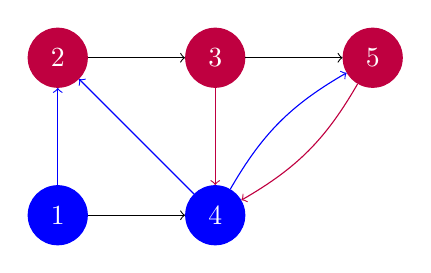
\begin{tikzpicture}[circle, node distance = 2cm, minimum size = 0.75cm]
      \node[draw, fill=purple, draw=purple, text=white] (2) {2};
      \node[draw, fill=purple, draw=purple, text=white] (3) [right of = 2] {3};
      \node[draw, fill=purple, draw=purple, text=white] (5) [right of = 3] {5};
      \node[draw, fill=blue, draw=blue, text=white] (1) [below of = 2] {1};
      \node[draw, fill=blue, draw=blue, text=white] (4) [below of = 3] {4};

      \path[->, color=blue] (1) edge (2);
      \path[->, color=blue] (4) edge (2);
      \path[->, color=blue] (4) edge [bend left=15] (5);

      \path[->, color=purple] (3) edge (4);
      \path[->, color=purple] (5) edge [bend left=15] (4);

      \path[->] (2) edge (3);
      \path[->] (3) edge (5);
      \path[->] (1) edge (4);
    \end{tikzpicture}
    \caption{incoming (\(\delta^+\)) and outgoing (\(\delta^-\)) cuts of two sets of nodes \textit{(purple and blue)}}
    \label{subfig:incoming-outgoing-cuts}
  \end{subfigure}
  \caption{Examples of graphs}
  \label{fig:examples-of-graphs}
\end{figure}

\subsubsection{Graphs representation}

Graphs are represented by:

\begin{itemize}
  \item Adjacency \textbf{matrix} \(\mathbf{A}\) of size \(n \times n\) if the graph is dense:
        \[ a_{ij} = \begin{cases} 1 \ &\text{if } (i, j) \in A\\ a_{i_j} &\text{otherwise}\end{cases} \]
  \item Adjacency \textbf{list} \(\mathbf{A}\) of size \(n\) if the graph is sparse
\end{itemize}

The same representation can be used for both directed and undirected graphs;
the adjacency matrix for an undirected graph is \textbf{symmetric}.

\bigskip
An example of a graph representation is shown in Figure~\ref{fig:graph-representation}.

\begin{figure}
  \begin{subfigure}{0.33\textwidth}
    \centering
    \begin{tikzpicture}[circle, node distance = 2cm, minimum size = 0.75cm]
      \samplegraph

      \path[->] (1) edge (2);
      \path[->] (1) edge (4);
      \path[->] (2) edge (3);
      \path[->] (3) edge (4);
      \path[->] (3) edge (5);
      \path[->] (4) edge (2);
      \path[->] (4) edge[bend left=15] (5);
      \path[->] (5) edge[bend left=15] (4);
    \end{tikzpicture}
    \caption{Graph}
  \end{subfigure}
  \begin{subfigure}{0.33\textwidth}
    \centering
    \(A = \begin{bmatrix}
      0 & 1 & 0 & 1 & 0 \\
      0 & 0 & 1 & 0 & 0 \\
      0 & 0 & 0 & 1 & 1 \\
      0 & 1 & 0 & 0 & 1 \\
      0 & 0 & 0 & 1 & 0
    \end{bmatrix}\)
    \caption{Adjacency matrix}
  \end{subfigure}
  \begin{subfigure}{0.33\textwidth}
    \centering
    \(\begin{matrix}
      S(1) = \left\{2, 4\right\} \\
      S(2) = \left\{3\right\}    \\
      S(3) = \left\{4, 5\right\} \\
      S(4) = \left\{2, 5\right\} \\
      S(5) = \left\{4\right\}
    \end{matrix}\)
    \caption{Adjacency list}
  \end{subfigure}
  \caption{Graph representation}
  \label{fig:graph-representation}
\end{figure}

\subsubsection{Graph reachability problem}

\textbf{Definition}:
given a directed graph \(G = (N, A)\) and a node \(s \in N\), find all nodes reachable from \(s\)

\bigskip
\textbf{Goal}
\begin{itemize}[label=\(\rightarrow\)]
  \item \textit{Input}: graph \(G = (N, A)\), described via successor lists, and a node \(s \in N\)
  \item \textit{Output}: subset \(M \subseteq N\) of nodes of \(G\) reachable from \(s\)
\end{itemize}

The goal is reached by an \textit{efficient} algorithm to solve the problem, with the following properties:
\begin{itemize}
  \item a \textbf{queue} \(Q\) of nodes not yet processed is kept by the algorithm
  \item the queue uses a \texttt{FIFO} policy
  \item the nodes exploration is performed in a \textbf{breadth-first} manner
\end{itemize}

\bigskip
\textbf{Algorithm}
The algorithm pseudocode is shown in Code~\ref{lst:graph-reachability}.

\begin{lstlisting}[style=custom, language=pseudocode, caption={Graph reachability}, label={lst:graph-reachability}]
Q := {s}
M := {}
while Q is not empty do
  u := node $\in$ Q
  Q := Q \ {u}
  M := M $\cup$ {u}
  for (u, v) $\in \ \delta^+(u)$ do
    if v $\notin$ M and v $\notin$ Q then
      Q := Q $\cup$ {v}
    end
  end
end
\end{lstlisting}

The algorithm stops when \(\delta^+(M) = \emptyset\) \textit{(when the outgoing cut of the set of nodes \(M\) is empty)};
\(\delta^-(M)\) is the set of arcs with head node in \(M\) and tail in \(N \setminus M\).

\paragraph{Complexity analysis}

At each iteration of the \texttt{\textbf{while}} loop:

\begin{enumerate}
  \item A node \(u\) is \textbf{removed} from the queue \(Q\) and \textbf{added} to the set \(M\)
  \item For all nodes \(v\) directly reachable from \(u\) and not already in \(M\) or \(Q\), \(v\) is added to \(Q\)
\end{enumerate}

Since each node \(u\) is inserted in \(Q\) at most once and each arch \((u,v)\) is considered at most once, the overall complexity is:
\[ \bigO{n+m} \quad n = |N|, \, m =|A|\]
For dense graphs, this value converges to \(\bigO{n^2}\).

\subsection{Subgraphs and Trees}

Let \(G = (N, E)\) be a graph.
Then:

\begin{itemize}
  \item \(G^\prime = (N^\prime, E^\prime)\) is a \textbf{subgraph} of \(G\) if \(N^\prime \subseteq N\) and \(E^\prime \subseteq E\)
  \item A \textbf{tree} \(G_T = (N^\prime, T)\) of \(G\) is a connected, acyclic, subgraph of \(G\)
  \item \(G_T = (N^\prime, T)\) is a \textbf{spanning tree} of \(G\) if it contains all the nodes \textit{(\(N^\prime = N\))}
  \item The \textbf{leaves} of a tree are the nodes with degree \(1\)
\end{itemize}

\bigskip
A representation of these concepts is shown in Figure~\ref{fig:subgraphs-trees}.

\begin{figure}
  \centering
  \begin{subfigure}[t]{0.995\textwidth}
    \centering
    \begin{tikzpicture}[circle, node distance = 2cm, minimum size = 0.75cm]
      \samplegraph
      \sampleedges
    \end{tikzpicture}
    \caption{Graph \(G\)}
  \end{subfigure}
  \bigskip
  \begin{subfigure}[t]{0.3\textwidth}
    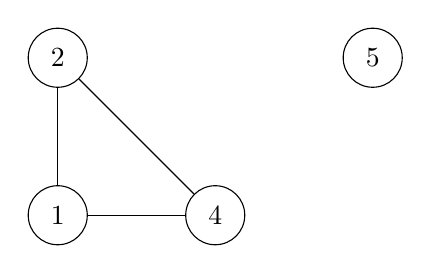
\begin{tikzpicture}[circle, node distance = 2cm, minimum size = 0.75cm]
      \node[draw] (2) {2};
      \node[] (3) [right of = 2] {};
      \node[draw] (5) [right of = 3] {5};
      \node[draw] (1) [below of = 2] {1};
      \node[draw] (4) [below of = 3] {4};

      \path[-] (2) edge (4);
      \path[-] (4) edge (1);
      \path[-] (1) edge (2);
    \end{tikzpicture}
    \caption{Subgraph \(G^\prime\) of \(G\)}
  \end{subfigure}
  \begin{subfigure}[t]{0.3\textwidth}
    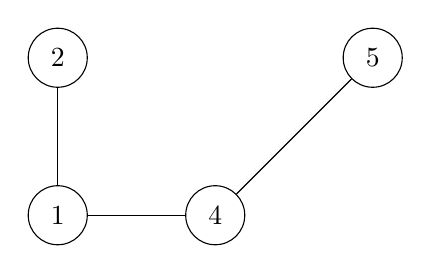
\begin{tikzpicture}[circle, node distance = 2cm, minimum size = 0.75cm]
      \node[draw] (2) {2};
      \node[] (3) [right of = 2] {};
      \node[draw] (5) [right of = 3] {5};
      \node[draw] (1) [below of = 2] {1};
      \node[draw] (4) [below of = 3] {4};

      \path[-] (5) edge (4);
      \path[-] (4) edge (1);
      \path[-] (1) edge (2);
    \end{tikzpicture}
    \caption{Subgraph \(G^{\prime\prime}\) of \(G\) and a tree}
  \end{subfigure}
  \begin{subfigure}[t]{0.3\textwidth}
    \begin{tikzpicture}[circle, node distance = 2cm, minimum size = 0.75cm]
      \samplegraph

      \path[-] (1) edge (4);
      \path[-] (2) edge (4);
      \path[-] (2) edge (3);
      \path[-] (4) edge (5);
    \end{tikzpicture}
    \caption{Subgraph \(G^{\prime\prime}\) of \(G\) and a tree}
  \end{subfigure}
  \caption{Subgraphs and trees}
  \label{fig:subgraphs-trees}
\end{figure}

\subsection{Properties of trees}

\subsubsection{Property 1 - number of edges}

Every tree with \(n\) nodes has \(n-1\) edges.

\paragraph{Proof}

\begin{itemize}
  \item \textbf{Base case}: the claim holds for \(n=1\) \textit{(a tree with a single node has no edges)}
  \item \textbf{Inductive steps}: show that the claim is valid for for any tree with \(n + 1\) nodes
        \begin{itemize}
          \item let \(T_1\) be a tree with \(n+1\) and recall with any tree with \(n \geq 2\) nodes has at least \(2\) leaves
          \item by deleting one of the leaves and its incident edge, a tree \(T_2\) with \(n\) nodes is obtained
          \item by induction hypothesis, \(T_2\) has \(n-1\) edges; therefore, \(T_1\) has \(n-1+1=n\) edges
        \end{itemize}
\end{itemize}

\subsubsection{Property 2 - number of paths}
\label{sec:property-2}

Any pair of nodes in a tree is connected via a unique path.

Otherwise, the tree would contain a cycle.

\subsubsection{Property 3 - new cycles}

By adding a new edge to a tree, a new unique cycle is created.
This cycle consists of the path in \nameref{sec:property-2} and the new edge.

\subsubsection{Property 4 - exchange property}

Let \(G_T = (N, T)\) be a spanning tree of \(G = (N, E)\).
Consider an edge \(e \notin T\) and the unique cycle \(C\) of \(T \cup \{e\}\).

For each edge \(f \in C \setminus \{e\}\), the subgraph \(T \cup \{e\} \setminus \{f\}\) is a spanning tree of \(G\).

\begin{figure}[htbp]
  \centering
  \bigskip
  \begin{subfigure}[t]{0.495\textwidth}
    \centering
    \begin{tikzpicture}[circle, node distance = 2cm, minimum size = 0.75cm]
      \samplegraph
      \path[-] (1) edge (2);
      \path[-] (2) edge (3);
      \path[-, text=red, color=red] (3) edge node[above]{\(f\)} (5);
      \path[-] (5) edge (4);
      \path[-, text=blue,color=blue] (4) edge node[above]{\(e\)} (2);
    \end{tikzpicture}
    \caption{Graph \(G_T\), edge \(f\) is red, edge \(e\) is blue}
  \end{subfigure}
  \begin{subfigure}[t]{0.495\textwidth}
    \centering
    \begin{tikzpicture}[circle, node distance = 2cm, minimum size = 0.75cm]
      \samplegraph

      \path[-] (1) edge (2);
      \path[-] (2) edge (3);
      \path[-] (3) edge (5);
      \path[-] (5) edge (4);
    \end{tikzpicture}
    \caption{\(T \cup \{e\} \setminus \{f\}\)}
  \end{subfigure}
  \caption{Exchange property}
  \label{fig:exchange-property}
  \bigskip
\end{figure}

\subsubsection{Property 5 - cut property}

Let \(F\) be a partial tree \textit{(spanning nodes in \(S \subseteq N\))} contained in a optimal spanning tree of \(G = (N, E)\).
Consider \(e = \left\{u, v\right\} \in \delta(S)\) of minimum cost, then there exists a minimum cost spanning tree of \(G\) containing \(e\).

\paragraph{Proof}

By contradiction, assume \(T^\ast \subseteq E\) is a minimum cost spanning tree with \(F \subseteq T^\ast\) and \(e \notin T^\ast\).

Adding an edge \(e\) to \(T^\ast\) creates the cycle \(C\).
Let \(f \in \delta(S) \cap C\):

\begin{itemize}
  \item If \(c_e = c_f\), then \(T^\ast \cup \{e\}\setminus \{f\}\) is a minimum cost spanning tree of \(G\) as it has the same cost as \(T^\ast\)
  \item If \(c_e < c_f\), then \(c \left( T^\ast \cup \{e\} \setminus \{f\} \right) < c \left(T^\ast\right)\), hence \(T^\ast\) is not optimal
\end{itemize}

\subsection{Optimal cost spanning tree}

\textbf{Spanning trees} have a number of applications:

\begin{itemize}
  \item \textbf{network} design
  \item \textbf{IP network} protocols
  \item \textbf{compact memory} storage
  \item \ldots
\end{itemize}

\bigskip
\textbf{Model}:
an undirected graph \(G = (N, E), \, n = |N|, \, m = |E|\) and a cost function \(c: E \rightarrow \mathbb{R}\), that assigns a cost to each edge, with \(e = \{u, v\} \in E\).

\bigskip
\textbf{Required properties}
\begin{enumerate}
  \item Each \textbf{pair of nodes} must be in a \textbf{path} \(\Rightarrow\) the output must be a \textbf{connected subgraph} containing all the nodes \(N\) of \(G\)
  \item The \textbf{subgraph} must have \textbf{no cycles} \(\Rightarrow\) the output must be a \textbf{tree}
\end{enumerate}

\bigskip
\textbf{Formalized problem}:
given an undirected graph \(G = (N, E)\) and a cost function \(c: E \rightarrow \mathbb{R}\), find a spanning tree \(G_T(N, T)\) of \(G\) of minimum, total cost.

The objective is finding:
\[ \displaystyle \min_{T \in X} \sum_{e \in T} c_e \qquad X = \text{ set of all spanning trees of } G \]

\subsubsection{Theorem 1 - number of nodes in spanning trees}

The \textbf{Theorem 1}, formulated by \textit{Cayley} in \(1889\), states that:

A complete graph with \(n\) nodes (\(n \geq 1\)) has \(n^{n-2}\) spanning trees.

\subsubsection{Prim's algorithm}

\textbf{Idea}: iteratively build a spanning tree.

\bigskip
\textbf{Method}
\begin{enumerate}
  \item Start from initial tree \((S, T)\) with \(S = \{u\}, S \subseteq N\) and \(T = \emptyset\)
  \item At each ste, add to the current partial tree \((S, T)\) an edge of minimum cost among those which connect a node in \(S\) to a node in \(N \setminus S\)
\end{enumerate}

\bigskip
\textbf{Goal}
\begin{itemize}[label=\(\rightarrow\)]
  \item \textit{Input}: connected graph \(G = (N, E)\) with edge costs.
  \item \textit{Output}: subset \(T \subseteq N\) of edges of \(G\) such that \(G_T = (N, T)\) is a minimum cost spanning tree of \(G\).
\end{itemize}

\bigskip
\textbf{Complexity}
if all edges are scanned at each iteration, the complexity order is \(\bigO{nm}\)

\bigskip
\textbf{Algorithm}
the pseudocode of the algorithm is shown in Code~\ref{lst:prims-algorithm}.

\begin{lstlisting}[style=custom, language=pseudocode, caption={Prim's algorithm}, label={lst:prims-algorithm}]
S := {u}
T := {}
while |T| < n - 1 do
  {u, v} := edge $\in\ \delta(S)$ with minimum cost // $u \in S, v \in N \setminus S$
  S := S $\cup$ {v}
  T := T $\cup$ {{u, v}}
end
\end{lstlisting}

\bigskip
Prim's algorithm is \textbf{greedy}:
at each step a minimum cost edge is selected among those in the cut \(\delta(S)\) induced by the current set of nodes \(S\).

\paragraph{Correcteness of Prim's algorithm}

\textbf{Proposition}: Prim's algorithm is exact.

The exactness does not depend on the choice of the first node nor on the selected edge of minimum cost \(\delta(S)\).
Each selected edge is part of the optimal solution as it belongs to a minimum spanning tree.

\paragraph{Optimality test}

The optimality condition allows to verify whether a spanning tree \(T\) is optimal or not;
it suffices to check that each \(e \in E \setminus T\) is not a cost decreasing edge.

\paragraph{Implementation in quadratic time}

The Prim's algorithm can be implemented in quadratic time \textit{(\(\bigO{n^2}\))}.

\bigskip
\textbf{Data structure}

\begin{itemize}
  \item \(k\) number of edges selected so far
  \item Subset \(S \subseteq N\) of nodes incident to the selected edges
  \item Subset \(T \subseteq E\) of selected edges
  \item \(C_j = \begin{cases} \min \{c_{ij} \, | \, i \in S\} \quad &j \notin S \\ +\infty &\text{otherwise}\end{cases}\)
  \item \(\textit{closest}_j = \begin{cases} \argmin\{c_{ij} \, | \, i \in S\}  & j \notin S \\ \text{predecessor of } j \text{ in the minimum spanning tree} \quad& j \in S \end{cases}\)
\end{itemize}

\bigskip
An example of a step is shown in Figure~\ref{fig:prim-quadratic-data-structure}.

\begin{figure}[htbp]
  \centering
  \bigskip
  \centering
  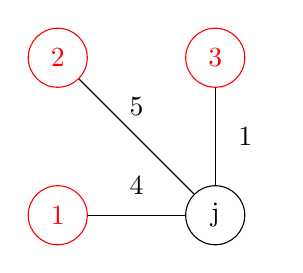
\begin{tikzpicture}[circle, node distance = 2cm, minimum size = 0.75cm]
    \node[draw=red, text=red] (2) {2};
    \node[draw=red, text=red] (3) [right of = 2] {3};
    \node[draw=red, text=red] (1) [below of = 2] {1};
    \node[draw] (j) [below of = 3] {j};

    \path[-] (1) edge node[above] {\(4\)} (j);
    \path[-] (2) edge node[above] {\(5\)} (j);
    \path[-] (3) edge node[right] {\(1\)} (j);
  \end{tikzpicture}
  \caption{Data structure}
  \label{fig:prim-quadratic-data-structure}
  \shortstack{
    nodes \(1, 2, 3 \in S\), node \(j \notin S\) \\
    \(\text{closest}_j = 3 \quad c_{\text{closest}_j j} = 1\)
  }
  \bigskip
\end{figure}

The spanning tree is built is built by selecting the node \(j\) with minimum cost \(C_j\) and adding the edge \(\{j, \textit{closest}_j\}\) to the spanning tree.

\bigskip
The code for this algorithm is shown in Code~\ref{lst:prim-quadratic}.

\begin{lstlisting}[style=custom, language=pseudocode, caption={Prim's algorithm in quadratic time}, label={lst:prim-quadratic}]
T := {}
S := {u}
// initialization
for j $\notin$ N $\setminus$ S do
  if {u, j} $\in$ E then
    C_j := c_{u, j}
  else
    C_j := +\infty
  end
  closest_j := u
end
for k := 1 to n - 1 do
  min := $+\infty$ // selection of min cost edge
  for j := 1, ..., n do
    if j $\notin$ S and C_j < min then
      min := C_j
      v := j
    end
  end
  S := S $\cup$ {v} // extend S
  T := T $\cup$ {{v, closest_v}} // extend T
  for j := 1 to n do
    if j $\notin$ S and c_vj < C_j then
      C_j := c_vj
      closest_j := v
    end
  end
end
\end{lstlisting}

\bigskip
The complexity of this algorithm is \(\bigO{n^2}\).
For sparse graphs, where \(m \ll \dfrac{n(n-1)}{2}\), a more efficient implementation (\(\bigO{m \log{(2)}}\)) \textit{(using priority queues)} is possible.

\subsubsection{Optimality condition}

Given a spanning tree \(T\), an edge \(e \notin T\) is cost decreasing if when added to \(T\), it creates a cycle \(C\) with \(C \subseteq T \cup \{e\}\) and \(\exists \, f \in C \setminus \{e\} \ \text{such that} \  c_e < c_f\).

\subsubsection{Theorem 2 - Tree optimality condition}

A tree \(T\) is of minimum total cost if and only if no cost decreasing edge exists.

\paragraph{Proof}

\begin{itemize}
  \item[\(\Rightarrow\)] If a \textbf{cost decreasing edge exists}, then \(T\) is \textbf{not of minimum total cost}
  \item[\(\Leftarrow\)] If \textbf{no cost decreasing edge exists}, then \(T\) is \textbf{of minimum total cost}
    \begin{itemize}
      \item let \(T^\ast\) be a minimum cost spanning tree of graph \(G\), found via by Prim's algorithm
      \item it can be verified that \(T^\ast\) can be iteratively (changing one edge at a time) transformed into \(T\) without changing the total cost
      \item thus, \(T\) is also optimal
    \end{itemize}
\end{itemize}

\subsection{Optimal paths}

\textbf{Optimal} (shortest, longest, \ldots) paths have a wide range of applications:

\begin{itemize}
  \item \textbf{Google Maps}, \textbf{GPS} navigators
  \item Planning and management of \textbf{transportation}, \textbf{electrical}, and \textbf{telecommunication} \textbf{networks}
  \item \textbf{Problem} planning
  \item \ldots
\end{itemize}

\bigskip
\textbf{Model}:
Given a directed graph \(G = (N, A)\) with a cost \(c_{ij} \in \mathbb{R}\) associated to each arc \((i, j) \in A\), and two nodes \(s\) and \(t\), determine a minimum cost \textit{(shortest)} path from \(s\) to \(t\).

\begin{itemize}
  \item Each value \(c_{i, j}\) represents the cost \textit{(or length, travel time, \ldots)} of arc \((i, j) \in A\)
  \item Node \(s\) is the origin \textit{(or source)}, node \(t\) is the destination \textit{(or sink)}
\end{itemize}

\bigskip
\textbf{Properties} of optimal paths:
\begin{itemize}
  \item A path \(\langle (i_1, i_2), (i_2, i_3), \ldots, (i_{k-1}, i_k)  \rangle\) is simple if no node is visited more than once
\end{itemize}

\subsubsection{Property 6 - shortest path}

If \(c_{ij} \geq 0\) for all \((i, j) \in A\), there is at least one shortest path that is simple.

\subsubsection{Dijkstra's algorithm}

\textbf{Idea}: consider the nodes in increasing order of length \textit{(cost)} of the shortest path from \(s\) to any one of the other nodes.

\bigskip
\textbf{Method}
\begin{itemize}
  \item To each \textbf{node} \(j \in N\), a \textbf{label} \(L_j\) is associated
        \begin{itemize}
          \item[\(\Rightarrow\)] at the end of the algorithm, this label will be the cost of the minimum cost path from \(s\) to \(j\)
        \end{itemize}
  \item Another label \(\textit{predecessor}_j\) is associated to each node \(j \in N\)
        \begin{itemize}
          \item[\(\Rightarrow\)] at the end of the algorithm, this label will be the node that precedes \(j\) on the minimum cost path from \(s\) to \(j\)
        \end{itemize}
  \item Make a \textbf{greedy} choice with respect to the paths from \(s\) to \(j\)
  \item A set of \textbf{shortest paths} from \(s\) to any node \(j \notin s\) can be retrieved backwards from \(t\) to \(s\) iterating over the predecessors
\end{itemize}

\bigskip
\textbf{Goal}
\begin{itemize}[label=\(\rightarrow\)]
  \item \textit{Input}: graph \(G = (N, A)\), cost \(c_{ij} \geq 0 \, \forall \, i, j\), origin \(s \in N\)
  \item \textit{Output}: shortest path from \(s\) to all other nodes in \(G\)
\end{itemize}

\bigskip
\textbf{Data structure}
\begin{itemize}
  \item \(S \subseteq N\): subset of nodes whose labels are permanent
  \item \(X \subseteq N\): subset of nodes with temporary labels
  \item \(L_j = \begin{cases} \text{cost of a shortest path from } s \text{ to } j \quad & j \in S \\ \min\{L_i + c_{ij} \, | \, (i, j) \in \delta^+(S) & j \notin S\}\end{cases}\)
        \begin{itemize}[label=\(\rightarrow\)]
          \item given a directed graph \(G\) and the current subset of nodes \(S \subset N\), consider the outgoing cut \(\delta^+(S)\) and select \((u, v) \in \delta^+(S)\) such that: \( L_u + c_{uv} = \min\{L_i + c_{ij} \, | \, (i, j) \in \delta^+ (S)\}\)
          \item thus: \(L_u + c_{uv} \leq L_i + c_{ij}, \forall \, (i, j) \in \delta^+(S)\)
        \end{itemize}
  \item \(\text{predecessor}_j = \begin{cases}\text{predecessor of } j \text{ in the shortest path from } s \text{ to } j \quad& j \in S \\ u \text{ such that } L_u + c_{uj} = \min\{L_i + c_{ij} \, | \, i \in S\} & j \notin S\end{cases}\)
\end{itemize}

\bigskip
\textbf{Complexity}:
the complexity of the algorithm depends on the how the arc \((u, v)\) is selected among those of the current cut \(\delta^+(u)\).
\begin{itemize}
  \item If all \(m\) arcs are scanned, the overall complexity would be \(\bigO{nm}\), hence \(\bigO{n^3}\)
  \item If all labels \(L_j\) are determined by appropriate updates (as in Prim's algorithm), only a single arc of \(\delta^+(j)\) is scanned, hence the complexity is \(\bigO{n^2}\)
\end{itemize}

\bigskip
\textbf{Notes}:
\begin{itemize}
  \item A set of shortest paths from \(s\) to all the nodes \(j \in N\) can be retrieved backwards from \(t\) to \(s\) iterating over the predecessors
  \item The union of a set of shortest paths from node \(s\) to all the other nodes of \(G\) is an arborescence rooted at \(s\)
  \item Dijkstra's algorithm does not work when there are arcs with negative cost: if \(G\) contains a circuit of negative cost, the shortest path problem may not be well defined
\end{itemize}

\bigskip
The code for this algorithm is shown in Code~\ref{lst:dijkstras-algorithm}.

\begin{lstlisting}[style=custom, language=pseudocode, caption={Dijkstra's algorithm}, label={lst:dijkstras-algorithm}]
S := {}
X := {s}
for u $\in$ N do
  L_u := $\infty$
end
L_s := 0
while |S| < |N| do
  u := argmin{L_i $|$ i $\in$ X}
  X := X $\backslash$ {u}
  S := S $\cup$ {u}
  for (u, v) $\in \delta^+(u)$ do
    if L_v > L_u + c_uv then
      L_v := L_u + c_uv
      predecessor_v := u
      X := X $\cup$ {v}
    end
  end
end
\end{lstlisting}

\paragraph{Correcteness of Dijkstra's algorithm}

Dijkstra's algorithm is correct.

\textbf{Proof}:
\begin{enumerate}
  \item A the \(k\)-th step:
        \begin{itemize}
          \item \(S = \{s, i_1, \ldots, i_{k-1}\}\)
          \item \(\begin{cases}\text{cost of a minimum cost path from } s \text{ to } j & j \in S \\ \text{cost of a minimum cost path with all intermediate nodes in } S \quad & j \notin S\end{cases}\)
        \end{itemize}
  \item By induction on the number \(k\) of steps:
        \begin{itemize}
          \item base case: for \(k = 1\) the statement holds, since
                \[S = \{s\}, \quad L_s = 0, \quad L_j = +\infty, \quad \forall \, j \notin S \]
          \item inductive step: assume that the statement holds for \(k+1\)
                \begin{itemize}
                  \item let \(u \notin S\) be the node that is inserted in \(S\) and \(\phi\) the path from \(s\) to \(u\) such that:
                        \[ L_v + c_{vu} \leq L_i + c_{iu}, \quad \forall \, (i, v) \in \delta^+(S) \]
                  \item every path \(\pi\) from \(s\) to \(u\) has \(c(\pi) \geq c(\phi)\), as there exists \(i \in S\) and \(j \notin S\) such that:
                        \[ \pi = \pi_1 \cup \left\{ \left( i, j \right)  \right\} \cup \pi_2 \]
                        where \((i, j)\) is the first arc in \(\pi \cap \delta^+(S)\)
                  \item it holds that
                        \[ c(\pi) = c(\pi_1) + c_{ij} + c(\pi_2) \geq L_i + c_{ij} \]
                        because \(c_{ij} \geq 0 \Rightarrow c(\pi_2) \geq 0\) and by the choice of \((v, u)\), \(c(\pi_1) \geq L_i\)
                  \item finally, by induction assumption:
                        \[ L_i + c_{ij} \geq L_v + c_{vu} = c(\phi) \]
                  \item a visualization of this step of the proof is shown in Figure~\ref{fig:proof-of-the-induction-step}
                \end{itemize}
        \end{itemize}
\end{enumerate}

\begin{figure}[htbp]
  \centering
  \bigskip
  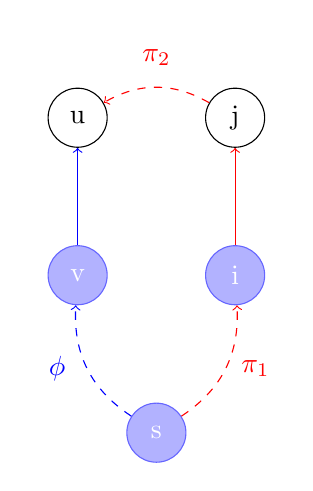
\begin{tikzpicture}[circle, node distance = 2cm, minimum size = 0.75cm]
    \node[draw] (u) at (-2, 0) {u};
    \node[draw] (j) at (0, 0) {j};
    \node[draw=blue!60, text=white, fill=blue!30] (v) at (-2, -2) {v};
    \node[draw=blue!60, text=white, fill=blue!30] (i) at (0, -2) {i};
    \node[draw=blue!60, text=white, fill=blue!30] (s) at (-1, -4) {s};

    \draw[dashed, ->, draw=blue] (s) edge[bend left] node[left, text=blue] {\(\phi\)} (v);
    \draw[dashed, ->, draw=red] (s) edge[bend right] node[right, text=red] {\(\pi_1\)} (i);
    \draw[->, draw=red] (i) edge (j);
    \draw[->, draw=blue] (v) edge (u);
    \draw[dashed, ->, draw=red] (j) edge[bend right] node[above, text=red] {\(\pi_2\)} (u);
  \end{tikzpicture}
  \caption{Proof of the induction step; nodes \(s, v, i\) are in cut \(S\)}
  \label{fig:proof-of-the-induction-step}
  \bigskip
\end{figure}

\paragraph{Example of Dijkstra's algorithm}

An example of Dijkstra's algorithm is shown in Figure~\ref{fig:dijkstra-example}.

\begin{figure}[tbp]
  \centering
  \bigskip
  \begin{subfigure}[t]{\textwidth}
    \centering
    \begin{tikzpicture}[circle, node distance = 2cm, minimum size = 0.75cm]
      \samplegraph

      \path[->] (1) edge node[left=-0.5mm] {5} (2);
      \path[->] (1) edge node[below=-0.5mm] {9} (4);
      \path[->] (2) edge[bend left=15] node[above=-1mm] {3} (3);
      \path[->] (2) edge node[left=-0.5mm] {2} (4);
      \path[->] (3) edge[bend left=15] node[below=-1mm] {1} (2);
      \path[->] (3) edge[bend left=15] node[right=-1mm] {0} (4);
      \path[->] (4) edge[bend left=15] node[left=-1mm] {2} (3);
      \path[->] (3) edge node[above=-0.5mm] {5} (5);
      \path[->] (4) edge node[below=-0.5mm] {9} (5);
    \end{tikzpicture}
    \caption{Sample graph, with the cost of each arc}
  \end{subfigure}
  \bigskip
  \begin{subfigure}[t]{0.32\textwidth}
    \centering
    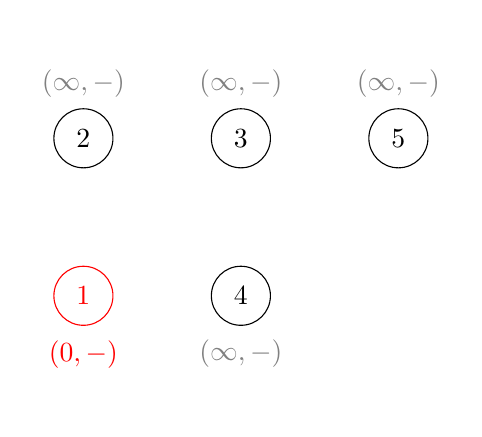
\begin{tikzpicture}[circle, node distance = 2cm, minimum size = 0.75cm]
      \node[draw, label={[text=gray, above=-0.4cm]\((\infty, -)\)}] (2) {2};
      \node[draw, label={[text=gray, above=-0.4cm]\((\infty, -)\)}] (3) [right of = 2] {3};
      \node[draw, label={[text=gray, above=-0.4cm]\((\infty, -)\)}] (5) [right of = 3] {5};
      \node[draw=red, text=red, label={[text=red, below=0.5cm]\((0, -)\)}] (1) [below of = 2] {1};
      \node[draw, label={[text=gray, below=0.4cm]\((\infty, -)\)}] (4) [right of = 1] {4};
    \end{tikzpicture}
    \caption{step 1 of Dijkstra's algorithm}
  \end{subfigure}
  \begin{subfigure}[t]{0.32\textwidth}
    \centering
    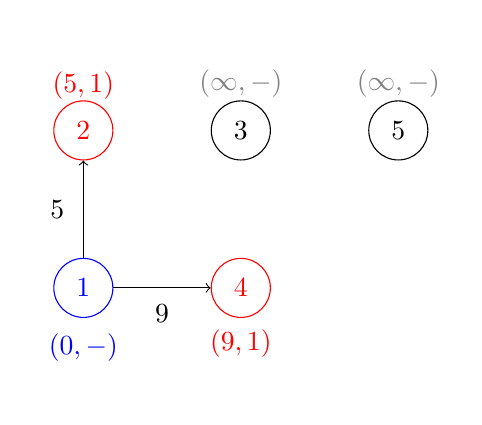
\begin{tikzpicture}[circle, node distance = 2cm, minimum size = 0.75cm]
      \node[draw=red, text=red, label={[text=red, above=-0.4cm]\((5, 1)\)}] (2) {2};
      \node[draw, label={[text=gray, above=-0.5cm]\((\infty, -)\)}] (3) [right of = 2] {3};
      \node[draw, label={[text=gray, above=-0.5cm]\((\infty, -)\)}] (5) [right of = 3] {5};
      \node[draw=blue, text=blue, label={[text=blue, below=0.5cm]\((0, -)\)}] (1) [below of = 2] {1};
      \node[draw=red, text=red, label={[text=red, below=0.5cm]\((9, 1)\)}] (4) [right of = 1] {4};

      \path[->] (1) edge node[left=-0.5mm] {5} (2);
      \path[->] (1) edge node[below=-0.5mm] {9} (4);
    \end{tikzpicture}
    \caption{step 2 of Dijkstra's algorithm}
  \end{subfigure}
  \begin{subfigure}[t]{0.32\textwidth}
    \centering
    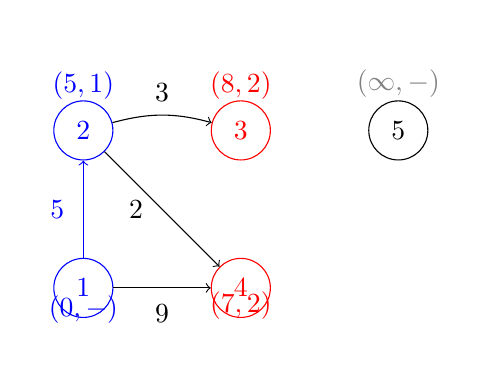
\begin{tikzpicture}[circle, node distance = 2cm, minimum size = 0.75cm]
      \node[draw=blue, text=blue, label={[text=blue, above=-0.4cm]\((5, 1)\)}] (2) {2};
      \node[draw=red, text=red, label={[text=red, above=-0.4cm]\((8, 2)\)}] (3) [right of = 2] {3};
      \node[draw, label={[text=gray, above=-0.5cm]\((\infty, -)\)}] (5) [right of = 3] {5};
      \node[draw=blue, text=blue, label={[text=blue, below = 0.5]\((0, -)\)}] (1) [below of = 2] {1};
      \node[draw=red, text=red, label={[text=red, below = 0.5]\((7, 2)\)}] (4) [right of = 1] {4};

      \path[->, blue] (1) edge node[left=-0.5mm] {5} (2);
      \path[->] (1) edge node[below=-0.5mm] {9} (4);
      \path[->] (2) edge[bend left=15] node[above=-1mm] {3} (3);
      \path[->] (2) edge node[left=-0.5mm] {2} (4);
    \end{tikzpicture}
    \caption{step 3 of Dijkstra's algorithm}
  \end{subfigure}
  \bigskip
  \begin{subfigure}[t]{0.32\textwidth}
    \centering
    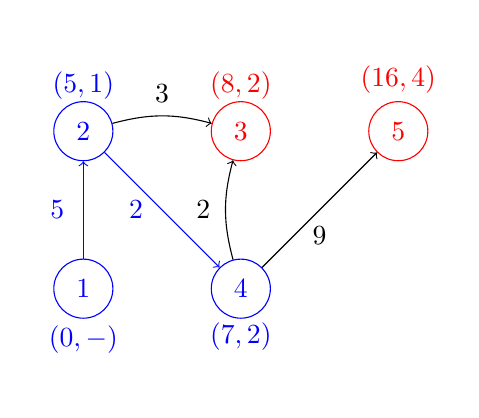
\begin{tikzpicture}[circle, node distance = 2cm, minimum size = 0.75cm]
      \node[draw=blue, text=blue, label={[text=blue, above=-0.4cm]\((5, 1)\)}] (2) {2};
      \node[draw=red, text=red, label={[text=red, above=-0.4cm]\((8, 2)\)}] (3) [right of = 2] {3};
      \node[draw=red, text=red, label={[text=red, above=-0.4cm]\((16, 4)\)}] (5) [right of = 3] {5};
      \node[draw=blue, text=blue, label={[text=blue, below=0.4cm]\((0, -)\)}] (1) [below of = 2] {1};
      \node[draw=blue, text=blue, label={[text=blue, below=0.4cm]\((7, 2)\)}] (4) [right of = 1] {4};

      \path[->, blue] (1) edge node[left=-0.5mm] {5} (2);
      \path[->] (2) edge[bend left=15] node[above=-1mm] {3} (3);
      \path[->, blue] (2) edge node[left=-0.5mm] {2} (4);
      \path[->] (4) edge[bend left=15] node[left=-1mm] {2} (3);
      \path[->] (4) edge node[below=-0.5mm] {9} (5);
    \end{tikzpicture}
    \caption{step 4 of Dijkstra's algorithm}
  \end{subfigure}
  \begin{subfigure}[t]{0.32\textwidth}
    \centering
    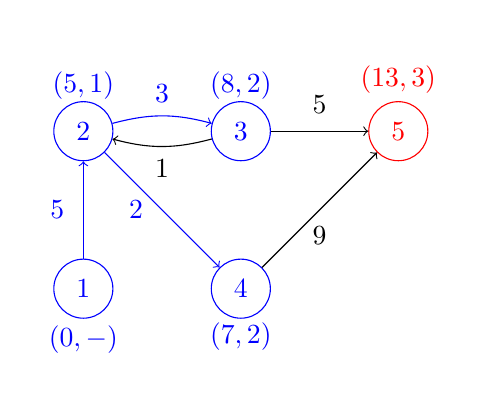
\begin{tikzpicture}[circle, node distance = 2cm, minimum size = 0.75cm]
      \node[draw=blue, text=blue, label={[text=blue, above=-0.4cm]\((5, 1)\)}] (2) {2};
      \node[draw=blue, text=blue, label={[text=blue, above=-0.4cm]\((8, 2)\)}] (3) [right of = 2] {3};
      \node[draw=red, text=red, label={[text=red, above=-0.4cm]\((13, 3)\)}] (5) [right of = 3] {5};
      \node[draw=blue, text=blue, label={[text=blue, below=0.4cm]\((0, -)\)}] (1) [below of = 2] {1};
      \node[draw=blue, text=blue, label={[text=blue, below=0.4cm]\((7, 2)\)}] (4) [right of = 1] {4};

      \path[->, blue] (1) edge node[left=-0.5mm] {5} (2);
      \path[->, blue] (2) edge[bend left=15] node[above=-1mm] {3} (3);
      \path[->, blue] (2) edge node[left=-0.5mm] {2} (4);
      \path[->] (3) edge[bend left=15] node[below=-1mm] {1} (2);
      \path[->] (3) edge node[above=-0.5mm] {5} (5);
      \path[->] (4) edge node[below=-0.5mm] {9} (5);
    \end{tikzpicture}
    \caption{step 5 of Dijkstra's algorithm}
  \end{subfigure}
  \begin{subfigure}[t]{0.32\textwidth}
    \centering
    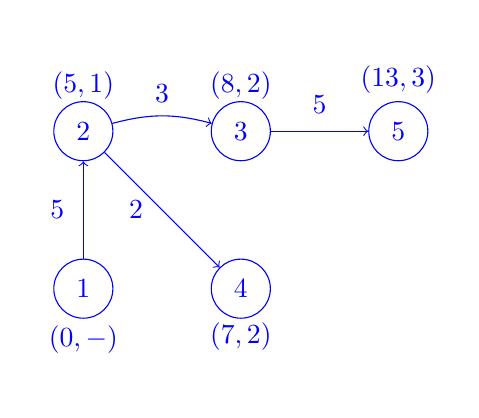
\begin{tikzpicture}[circle, node distance = 2cm, minimum size = 0.75cm]
      \node[draw=blue, text=blue, label={[text=blue, above=-0.4cm]\((5, 1)\)}] (2) {2};
      \node[draw=blue, text=blue, label={[text=blue, above=-0.4cm]\((8, 2)\)}] (3) [right of = 2] {3};
      \node[draw=blue, text=blue, label={[text=blue, above=-0.4cm]\((13, 3)\)}] (5) [right of = 3] {5};
      \node[draw=blue, text=blue, label={[text=blue, below=0.4cm]\((0, -)\)}] (1) [below of = 2] {1};
      \node[draw=blue, text=blue, label={[text=blue, below=0.4cm]\((7, 2)\)}] (4) [right of = 1] {4};

      \path[->, blue] (1) edge node[left=-0.5mm] {5} (2);
      \path[->, blue] (2) edge[bend left=15] node[above=-1mm] {3} (3);
      \path[->, blue] (2) edge node[left=-0.5mm] {2} (4);
      \path[->, blue] (3) edge node[above=-0.5mm] {5} (5);
    \end{tikzpicture}
    \caption{step 6 of Dijkstra's algorithm}
  \end{subfigure}
  \caption{Example of Dijkstra's algorithm}
  \label{fig:dijkstra-example}
\end{figure}

\subsubsection{Floyd-Warshall's algorithm}

\textbf{Goal}
\begin{itemize}[label=\(\rightarrow\)]
  \item \textit{Input}: a directed graph \(G = (N, A)\) with an \(n \times n\) cost matrix \(C = [c_{ij}]\)
  \item \textit{Output}: for each pair of nodes \(i, j \in N\), the cost \(c_{ij}\) of the shortest path from \(i\) to \(j\)
\end{itemize}

\bigskip
\textbf{Data structure}
\begin{itemize}
  \item Two \(n \times n\) matrices \(D, P\) whose elements correspond, at the end of the algorithm, to:
        \begin{itemize}
          \item[\(d_{ij}\)] the cost of the shortest path from \(i\) to \(j\)
          \item[\(p_{ij}\)] the predecessor of \(j\) on the shortest path from \(i\) to \(j\)
        \end{itemize}
\end{itemize}

\bigskip
\textbf{Method}
\begin{enumerate}
  \item Initialization of \(D\) and \(P\):
        \[ p_{ij} = i \quad \forall \, i \]
        \[ d_{ij} = \begin{cases} 0 \quad & i = j \\ c_{ij} & i \neq j \land (i, j) \in A \\ +\infty & \text{otherwise}  \end{cases} \]
  \item Triangular operation: for each pair of nodes \(i, j\), where \(i \neq u, j \neq u\), check whether the path from \(i\) to \(j\) is shorter by going through \(u\) (i.e. \(d_{iu} + d_{uj} < d_{ij}\))
\end{enumerate}

\bigskip
\textbf{Complexity}
\begin{itemize}
  \item Since in the worst case the triangular operation is executed for all nodes \(u\) ad for each pair of nodes \(i, j\), the complexity is \(\bigO{n^3}\)
\end{itemize}

\bigskip
The code for this algorithm is shown in Code~\ref{lst:floyd-warshall-algorithm}.

\begin{lstlisting}[style=custom, language=pseudocode, caption={Floyd-Warshall's algorithm}, label={lst:floyd-warshall-algorithm}]
for i := 1 to n do
  for j := 1 to n do
    p_id := i

    if i = j then
      d_ij := 0
    else if (i, j) in A then
      d_ij := c_ij
    else
      d_ij := $+\infty$
    end
  end
end
for u $\in$ N do
  for i $\in$ N $\setminus\{$ u $\}$ do
    for j $\in$ N $\setminus\{$ u $\}$
      if d_iu + d_uj < d_ij then
        p_ij := p_uj
        d_ij := d_iu + d_uj
      end
    end
  for i $\in$ N do
    if d_ij < 0 then
      error "negative cycle"
    end
end
\end{lstlisting}

\paragraph{Correctness of Floyd-Warshall's algorithm}

Floyd-Warshall's algorithm is correct.

\textbf{Proof}: assume that the nodes of \(G\) are numbered from \(1\) to \(n\).
Verify that, if the node index order is followed, after the \(u\)-th cycle the value \(d_{ij}\) \textit{(for any \(i, j\))} corresponds to the cost of a shortest path from \(i\) to \(j\) with at most \(u\) intermediate nodes (\(\left\{ 1, \ldots, u \right\}\))

\subsection{Optimal paths in directed, acyclic graphs}

A directed graph \(G = (N, A)\) is \textbf{acyclic} if it does not contain any circuit.
A directed acyclic graph \(G\) is then referred to as a \textbf{\DAG}.

Property of \textit{\DAGs}: the nodes of any directed acyclic graph \(G\) can be ordered topologically, i.e. indexed so that for each arc \((i, j) \in A\) the index of \(i\) is less than the index of \(j\) \textit{(\(i \leq j\))}.
The topological order can be exploited by dynamic programming algorithms to compute efficiently the shortest paths in a \DAG.

\textbf{Problem}: given a \DAG \(G = (N, A)\) with a cost \(c_{ij} \in \mathbb{R}\) and nodes \(s, t\), determine the shortest (or longest) path from \(s\) to \(t\).

\subsubsection{Topological ordering method}

The method requires \(G = (N, A)\) to be a \DAG represented via the list of predecessors \(\delta^-(v)\) and the list of successors \(\delta^+(v)\) of each node \(v \in N\).
Then, it works as follows:

\begin{enumerate}[label=\arabic*., ref=(\arabic*)]
  \item\label{enum:topological-ordering-1} Assign the smallest positive integer not yet assigned to a node \(v \in N \) with \(\delta^-(v) = \emptyset\)
  \begin{itemize}[label=\(\rightarrow\)]
    \item such node always exists because \(G\) does not contain circuits
  \end{itemize}
  \item Delete the node \(v\) with all its incident arcs
  \item Go to step  \ref{enum:topological-ordering-1} until all nodes have been assigned a number
\end{enumerate}

\begin{figure}[htbp]
  \centering
  \bigskip
  \begin{subfigure}[t]{0.495\textwidth}
    \centering
    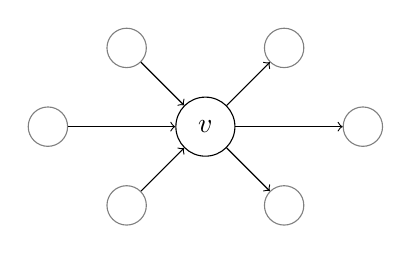
\begin{tikzpicture}[circle]
      \node[draw, circle, minimum size=0.75cm] (v) at (0, 0) {\(v\)};
      \node[draw=gray,circle, minimum size=0.5cm] (0) at (-1, -1) {};
      \node[draw=gray,circle, minimum size=0.5cm] (1) at (-2, 0) {};
      \node[draw=gray,circle, minimum size=0.5cm] (2) at (-1, 1) {};
      \node[draw=gray,circle, minimum size=0.5cm] (3) at (1, -1) {};
      \node[draw=gray,circle, minimum size=0.5cm] (4) at (2, 0) {};
      \node[draw=gray,circle, minimum size=0.5cm] (5) at (1, 1) {};

      \draw[->] (0) -- (v);
      \draw[->] (1) -- (v);
      \draw[->] (2) -- (v);

      \draw[->] (v) -- (3);
      \draw[->] (v) -- (4);
      \draw[->] (v) -- (5);
    \end{tikzpicture}
    \caption{Topological ordering}
    \label{fig:topological-ordering}
  \end{subfigure}
  \begin{subfigure}[t]{0.495\textwidth}
    \centering
    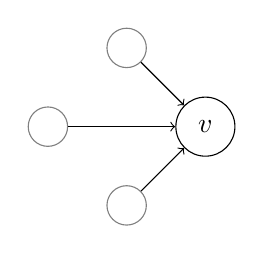
\begin{tikzpicture}[circle]
      \node[draw, circle, minimum size=0.75cm] (v) at (0, 0) {\(v\)};
      \node[draw=gray,circle, minimum size=0.5cm] (0) at (-1, -1) {};
      \node[draw=gray,circle, minimum size=0.5cm] (1) at (-2, 0) {};
      \node[draw=gray,circle, minimum size=0.5cm] (2) at (-1, 1) {};

      \draw[->] (0) -- (v);
      \draw[->] (1) -- (v);
      \draw[->] (2) -- (v);
    \end{tikzpicture}
    \caption{Node \(v\) with \(\delta^-(v) = \emptyset\), as in step \ref{enum:topological-ordering-1} of the algorithm}
    \label{fig:node-with-empty-successors}
  \end{subfigure}
  \caption{Topological ordering method}
  \label{fig:topological-ordering-method}
  \bigskip
\end{figure}

\bigskip
This algorithm has complexity \(\bigO{|A|}\), because each node is assigned a number only once.
Furthermore, all arcs incident to a node are deleted only once.

\subsubsection{Dynamic programming for shortest path in \DAGs}

Any shortest path from \(1\) to \(t\), called \(\pi_t\), with at least \(2\) arcs can be subdivided into two parts:

\begin{itemize}
  \item \(\pi_i\), the shortest subpath from \(s\) to \(i\)
  \item \(\left( i, t \right)\), the remaining part
\end{itemize}

This decomposition is called the optimality principle of shortest paths in \DAGs.
An illustration of this decomposition is shown in Figure \ref{fig:shortest-path-in-DAG}.

\begin{figure}[htbp]
  \centering
  \bigskip
  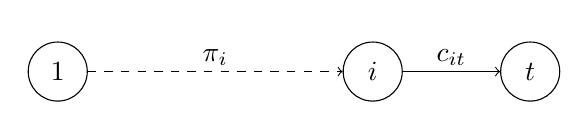
\begin{tikzpicture}[circle, minimum size = 0.75cm]
    \node[draw, circle] (1) at (-1, 0) {\(1\)};
    \node[draw, circle] (i) at (3, 0) {\(i\)};
    \node[draw, circle] (t) at (5, 0) {\(t\)};

    \draw[] (1) edge[dashed, ->] node[above=-0.2cm] {\(\pi_i\)} (i);
    \draw[->] (i) edge node[above=-0.2cm] {\(c_{it}\)} (t);
  \end{tikzpicture}
  \caption{Shortest path from \(1\) to \(t\)}
  \label{fig:shortest-path-in-DAG}
  \bigskip
\end{figure}

\bigskip
The strategy to find the shortest path is:

\begin{enumerate}
  \item For each node \(i = 1, \ldots, t\) let \(L_i\) be the cost of a shortest path from \(1\) to \(i\)
        \begin{itemize}[label=\(\rightarrow\)]
          \item \(L_t = \displaystyle \min_{(i, t) \in \delta^-(t)} \left\{ L_i + c_{it} \right\}\)
          \item the minimum is taken over all possible predecessors \(i\) of \(t\)
        \end{itemize}
  \item If \(G\) is topologically ordered \DAG, then the only possible predecessors of \(t\) in a shortest path \(\pi_t\) from \(1\) to \(t\) are those with index \(i < t\)
        \begin{itemize}[label=\(\rightarrow\)]
          \item \(L_t = \displaystyle \min_{i < t} \left\{ L_i + c_{it} \right\}\)
          \item in a graph with circuits, any node \(i\) can be a predecessor of \(t\) if \(i \neq t\)
        \end{itemize}
\end{enumerate}

For \DAGs whose nodes are topologically ordered \(L_{t-1}, \ldots, L_1\) satisfy the same type of recursive relations:

\[ L_{t-1} = \displaystyle \min_{i < t-1} \left\{ L_i + c_{i, t-1} \right\}; \ldots; L_2 = \displaystyle \min_{i=1}\left\{ L_i + c_{i2} \right\} = L_1 + c_{12}; L_1 = 0 \]
which can be solved in reversed order
\[ L_1 = 0; L_2 = L_1 + c_{12}; \ldots; L_{t} = \displaystyle \min_{i < t - 1} \left\{ L_i + c_t \right\} \]

\bigskip
\textbf{Algorithm}:
finally, the algorithm is shown in pseudocode in Algorithm~\ref{lst:shortest-path-in-DAG}.

\begin{lstlisting}[style=custom, language=pseudocode, caption={Shortest path in \DAG}, label={lst:shortest-path-in-DAG}]
sort the nodes of G topologically
L_1 := 0
for j := 2 to n do
  L_j := min{L_i + c_{ij} | (i, j) $\in \delta^-(\texttt{j}) \land \texttt{i} < \texttt{j}$}
  pred_j := v such that (v, j) = argmin{L_i + c_{ij} | (i, j) $\in \delta^-(\texttt{j}) \land \texttt{i} < \texttt{j}$}
\end{lstlisting}

\bigskip
Complexity of the algorithm is \(\bigO{|A|}\):

\begin{itemize}
  \item Topological ordering of the nodes: \(\bigO{m}\) with \(m = |A|\) (number of arcs)
  \item Each node/arc is processed only once: \(\bigO{n+m}\)
\end{itemize}

\bigskip
In order to find the longest path, the algorithm can be adapted as follows:
\[L_t = \displaystyle \max_{i < t} \left\{ L_i + c_{it} \right\}\]

\paragraph{Optimality of the algorithm}

The Dynamic Programming algorithm for finding shortest or longest paths in \DAGs is exact.
This is due to the optimality principle, already explored in the previous section.

\subsection{Project planning}

A project consists of a set of \(m\) activities with their (estimated) duration: activity \(A_i\) has duration \(d_i \geq 0, i = 1, \ldots, m\).
Some pair of activities allow a precedent constraint: \(A_i \propto A_j\) indicated that \(A_i\) must be performed before \(A_j\).

\textbf{Model}:
a project can be represented by a directed graph \(G = (N, A)\) where:

\begin{itemize}
  \item each arc corresponds to an activity
  \item the arc length represent the duration of the corresponding activity
\end{itemize}

In order to account for precedence constraints, the arcs must be positioned such that for activities \(A_i \propto A_j\) there exists a directed path where the arc associated to \(A_i\) precedes the arc associated to \(A_j\).
Such notation is shown in Figure \ref{fig:precedence-relation-in-project-planning}.

\begin{figure}[htbp]
  \centering
  \bigskip
  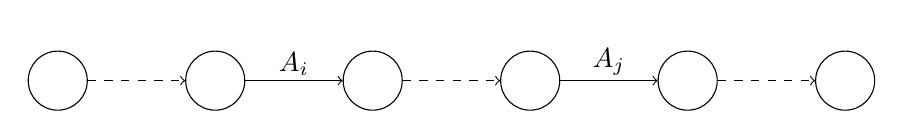
\begin{tikzpicture}[circle, node distance = 2cm, minimum size = 0.75cm]
    \node[draw] (1) {};
    \node[draw] (2) [right of = 1] {};
    \node[draw] (3) [right of = 2] {};
    \node[draw] (4) [right of = 3] {};
    \node[draw] (5) [right of = 4] {};
    \node[draw] (6) [right of = 5] {};

    \draw[dashed, ->] (1) edge (2);
    \draw[->] (2) edge node[above=-0.2cm]{\(A_i\)} (3);
    \draw[dashed, ->] (3) edge (4);
    \draw[->] (4) edge node[above=-0.2cm]{\(A_j\)} (5);
    \draw[dashed, ->] (5) edge (6);
  \end{tikzpicture}
  \bigskip
  \caption{Precedence relation in project planning}
  \label{fig:precedence-relation-in-project-planning}
\end{figure}

Therefore, a nove \(v\) marks an event corresponding to the end fo all the activities \(\left( i, v \right) \in \delta^-(v)\) and the (possible) start of all the activities \(\left( v, j \right) \in \delta^+(v)\).

\subsubsection{Property 7}

The directed graph \(G\) representing a project is acyclic \textit{(is a \DAG)}.

Proof:
by contradiction, if \(A_{i1} \propto A_{12} \propto \ldots \propto A_{jk} \propto A_{kj}\) there would be a logical inconsistency.

\subsubsection{Optimal paths}

A graph \(G\) can be simplified by contracting some arcs, but it's important to not introduce unwanted precedence constraints.
Artificial nodes or artificial arcs are introduced so that graph \(G\):

\begin{itemize}
  \item Contains a unique initial node \(s\) corresponding to the event \inlinequote{beginning of the project}
  \item Contains a unique final node \(t\) corresponding to the event \inlinequote{end of the project}
  \item does not contain multiple arcs with the same origin and destination
\end{itemize}

\bigskip
\textbf{Problem}:
given a project (set of activities with duration and precedence constraints), schedule the activities in order to minimize the overall project duration (the time needed to complete all the activities).

\paragraph{Property 8}

The minimum overall project duration is the length of a longest path from \(s\) to \(t\) in the graph \(G\).

\textbf{Proof}:
since any \(s-t\) path represents a sequence of activities that must be executed in the specified order, its length provides a lower bound on the minimum overall project duration.

\paragraph{Critical path method - \CPM}

The critical path method (\CPM) determines:

\begin{itemize}
  \item A schedule \textit{(a plan for executing the activities specifying the order and the assigned time)} that minimizes the overall project duration
  \item The slack of each activity \textit{(the amount of time by which its execution can be delayed without affecting the overall minimum project duration)}
\end{itemize}

\bigskip
\textbf{Initialization}:
construct the graph \(G\) representing the project.

\bigskip
\textbf{Method}:

\begin{enumerate}
  \item Find a topological order of the nodes
  \item Consider the nodes by increasing indices and for each \(h \in N\) find the earliest time \(T_{min_h}\) at which the event associated to node \(h\) can occur
  \begin{itemize}[label = \(\rightarrow\)]
    \item \(T_{min_h}\) corresponds to the minimum project duration
  \end{itemize}
  \item Consider the nodes by decreasing indices and for each \(h \in N\) find the latest time \(T_{max_h}\) at which the event associated to node \(h\) can occur without delaying the project completion date beyond \(T_{min_n}\)
  \item For each activity \(\left( i, j \right) \in A\) find the slack
  \begin{itemize}[label = \(\rightarrow\)]
    \item the slack is calculated as \(\sigma{ij} - T_{max_j}  - T_{min_i} - d_{ij}\)
  \end{itemize}
\end{enumerate}

\bigskip
\textbf{Input}:
graph \(G = (N, A)\) with \(n = |N|\) and the duration \(d_{ij}\) associated to each \(\left( i, j \right) \in A\)/

\textbf{Output}:
\(\left( T_{min_i}, T_{max_i} \right), i = 1, \ldots, n\)

\bigskip
\textbf{Algorithm}:
finally, the algorithm is shown in pseudocode in Algorithm~\ref{lst:critical-path-method}.

\begin{lstlisting}[style=custom, language=pseudocode, caption={Critical path method}, label={lst:critical-path-method}]
Sort the nodes topologically
T_min_i := 0
for j = 2 to n do
  T_min_j := max{T_min_i + d_ij | (i, j) $\in \delta^- (\texttt{j})$}
end for
T_max_n := T_min_n // minimum project duration
for i = n-1 to 1 do
  T_max_i := min{T_max_j - d_ij | (i, j) $\in \delta^+ (\texttt{i})$}
end for
\end{lstlisting}


\bigskip
\textbf{Complexity}:
the overall complexity is \(\bigO(n+m) \approx \bigO(m)\), due to the sum of

\begin{itemize}
  \item complexity of the topological sort - \(\bigO(n+m)\)
  \item complexity of the first loop - \(\bigO(n+m)\)
  \item complexity of the second loop - \(\bigO(n+m)\)
\end{itemize}

\paragraph{Critical paths}

An activity \(\left( i, j \right)\) with zero slack \(\sigma_{ij} = T_{max_j} = T_{min_i} = d_{ij} = 0\) is called \textbf{critical}.

A critical path is a path in a \(s-t\) composed uniquely by critical activities.
At least one always exists.

\paragraph{Gantt charts}

A Gantt chart is a graphical representation of a project schedule.
It was introduced in 1896 by Henry Gantt, an American mechanical engineer and management consultant.

There are two types of Gantt charts:

\begin{itemize}
  \item Gantt chart at earliest - each activity \(\left( i, j \right)\) starts at \(T_{min_i}\) and ends at \(T_{min_i} + d_{ij}\)
  \item Gantt chart at latest - each activity \(\left( i, j \right)\) starts at \(T_{max_i}\) and ends at \(T_{max_i} + d_{ij}\)
\end{itemize}

\end{document}